\documentclass{article}
\usepackage{blindtext}
\usepackage[a4paper, total={6in, 9in}]{geometry}

\usepackage{amsmath,amsfonts,graphicx} %math packages
\usepackage{listings,xcolor} %code snippet packages
\usepackage{setspace} %allows spaces to be set
\usepackage{tabularx} %flexible width tables
\usepackage{multicol} %enables multiple columns
\usepackage{enumitem} %customized lists
\usepackage[skip=5pt]{parskip} %flexible paragraph spacing options
\usepackage{csquotes} %quotations

\title{CS246e Final Design}
\author{Ray Wang}
\date{\today}

%\setstretch{1} %set line spacing to 1.25 
\setlength{\parindent}{0pt} %remove leading space in paragraphs
\pagestyle{empty} %empties the heading and footer 
\renewcommand{\arraystretch}{0.7} %table row spacing

\newcommand{\question}[1]{\section*{Question #1}}

\newcommand{\qpart}[1]{\subsection*{Part (#1)}}
\newenvironment{myitemize}
{ \begin{itemize}
    \setlength{\itemsep}{2pt}
    \setlength{\parskip}{0pt}
    \setlength{\parsep}{0pt}     }
{ \end{itemize}                  }

\begin{document}
\pagenumbering{arabic} %reset page numbering to default 
\section{Overview}
\quad The overall structure consists of a {\texttt src} folder containing main "Closures",
which together parse the command arguments (such as flags and files), 
setup ncurses, 
initialize the models, views, and controllers from lib, 
and create the connections between them.
These Closures are collected in a \texttt{Main} struct, 
which has a {\texttt main()} method to start the main loop.
In the actual main function, I 
initialize a Main struct, 
check if we need to print a help message, and if not, 
then execute \texttt{main()} in a try catch clause, returning 1 if an exception is caught.
Finally, for cleanup all Closures are RAIId so that 
destructors will cleanup the objects and processes they initialized 
(for example, \texttt{src/init\_ncurses.h} runs \texttt{endwin()}).

\quad The main loop starts by rendering the view (window, cursor, statusbar), 
waits for the user to type a key, then notifies the keyboard's observers. 
This repeats until the root window is closed (e. g. by \texttt{:wq}).
The user's input is converted by the 
\texttt{UWSEKeyboard} class (i.e. the view in MVC) 
into a \texttt{KeyStroke}, 
which is then consumed by a \texttt{ModeManager} 
(i.e. the first part of the model in MVC).
This manager contains the current \texttt{ModeType}, and forwards the keystroke to 
the \texttt{CommandParser}s corresponding to the current mode. 
The parsers will turn keystrokes into \texttt{Command}s. 
For example, \texttt{ComboNMParser} turns \texttt{4d2w} into 
\verb)ComboNM{{4,'d','\0'},{2,'w','\0'}}). 
Once a parser fully parses a \texttt{Command}, they notify their observers
(i.e. \texttt{CommandRunner}s) which update the rest of the model as needed. 
All of the things that runners will modify are: 
\begin{myitemize}
  \item{\texttt{ModeManager} - contains current \texttt{ModeType}. 
    Also will forward \texttt{KeyStroke}s from \texttt{MacroRunner}}
  \item{\texttt{LinedFilebuf} 
    - opens contents of a file from its filename 
    into an in-memory buffer with line-based editing operations. 
  \texttt{FstreamLFB} is a concrete implementation using \texttt{std::fstream}}
  \item{ \texttt{FileManager} 
    - maps each filename to its corresponding \texttt{LinedFilebuf}}
  \item{ \texttt{Cursor} 
      - current location (line, col) of the cursor in the \texttt{LinedFilebuf} }
  \item{ \texttt{Tab}
    - combines a \texttt{Cursor} and a \texttt{LinedFilebuf}. 
    Provides operations to synchronize \texttt{Cursor} with the window pane, 
  e.g. scrolling the window when cursor moves, and vice-versa}
  \item{ \texttt{TabManager} 
    - provides operations to move forwards and backwards in multi-file editing}
  \item{ \texttt{Clipboard}, \texttt{MacrosRegister} 
    - stores clipboard data and macro recordings, respectively}
  \item{ \texttt{RootStatus} - stores current message and/or error-code. 
    e.g. E37: file not written}
  \item{\texttt{Window} 
    - contains a \texttt{TabManager}. Provides operations for split-screening}
  \item{\texttt{HistoryTree} 
    - stores snapshots of a \texttt{LinedFilebuf}'s contents; 
    provides \texttt{undo}, \texttt{redo}}
  \item{\texttt{HistoryManager} 
    - Maps filenames to their corresponding \texttt{HistoryTree}s}
\end{myitemize}
\quad The view consists of a \texttt{NCWindow} which overrides the 
\texttt{render()} of \texttt{Window} to render in \texttt{ncurses}. 
It has 2 helpers: \texttt{StatusBar} and \texttt{Textbox}
which render the current \texttt{Tab}'s cursor location, 
and the contents of the \texttt{LinedFilebuf}. 
The view also has a \texttt{NCCursor} which renders the on-screen cursor. 
Its position is calculated based on the \texttt{Cursor} and \texttt{Tab} 
by \texttt{Main} via the \texttt{CursorClosure}. 
Finally, the view has a \texttt{RootStatusRender} 
which renders a \texttt{string} at the bottom left of the screen. 
The message it displays is calculated from \texttt{RootStatus} 
by \texttt{Main} via \texttt{StatusBarClosure}'s 
\texttt{render()} method.  

\section{Updated UML}
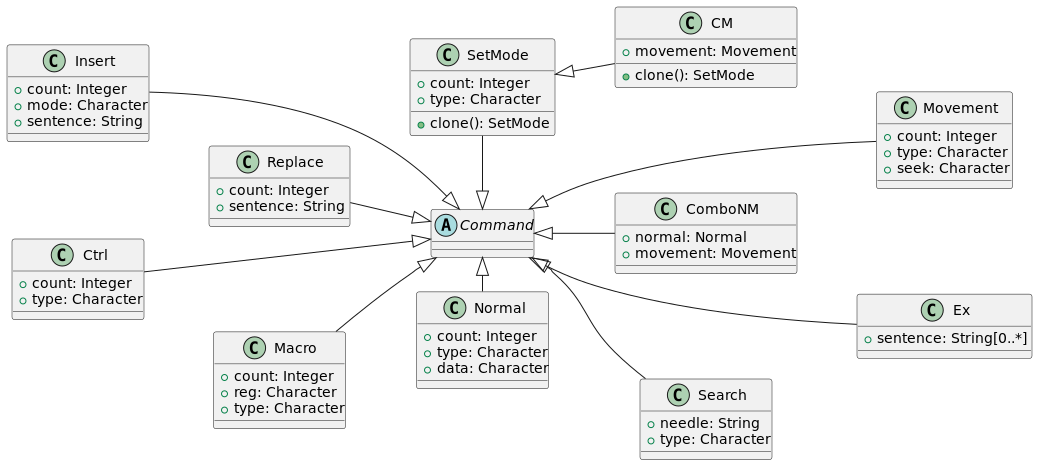
\includegraphics[width=\textwidth]{uml1}
Figure 1. Command Heirarchy updated to include \texttt{CM}, 
\texttt{Search}, and any renamed fields. 
\\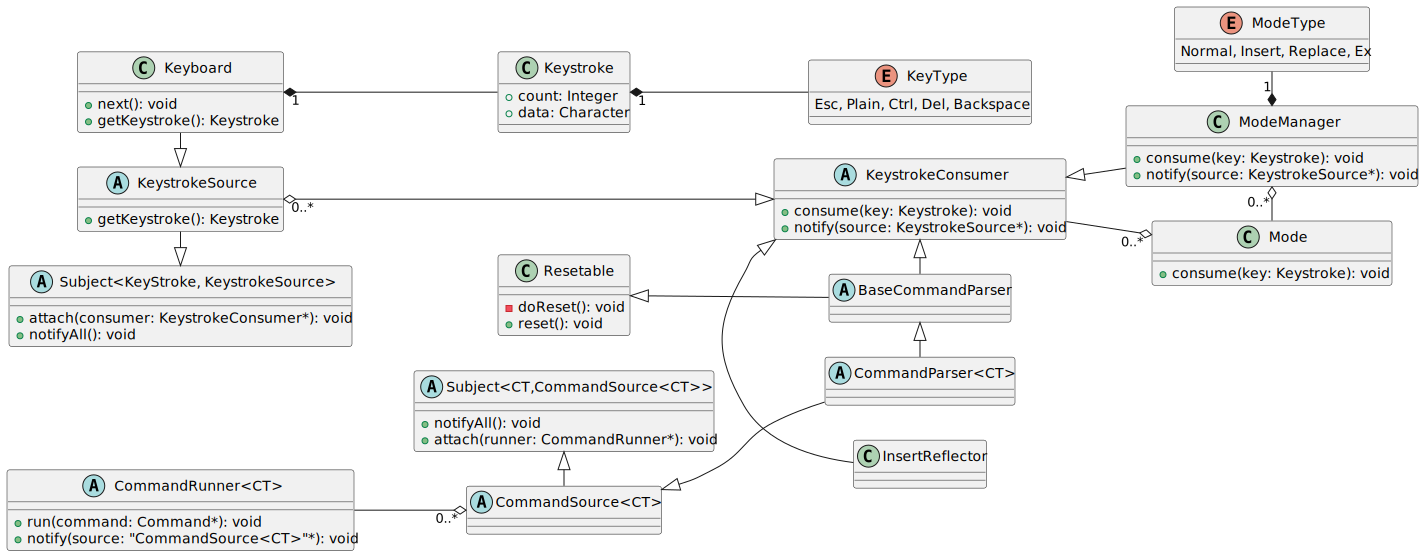
\includegraphics[width=\textwidth]{uml2}
Figure 2. Subjects and objects for \texttt{KeyStroke}s and 
\texttt{Command}, including their templates (see \textbf{Observer Patter})
\\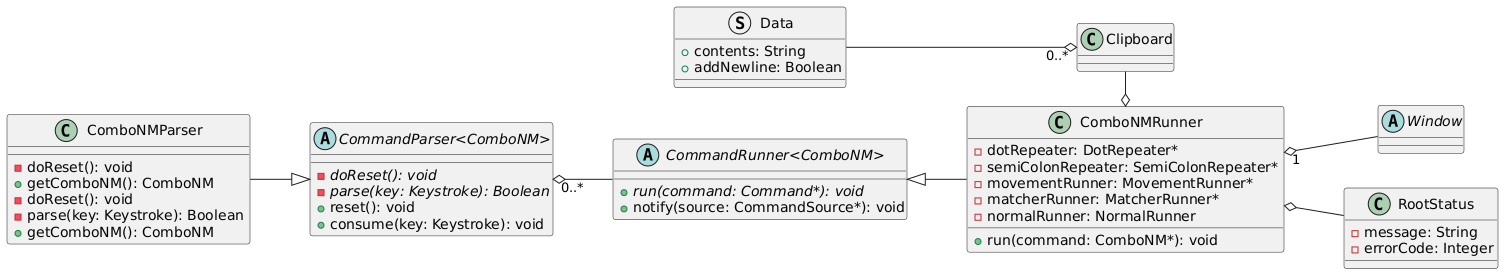
\includegraphics[width=\textwidth]{uml4}
\\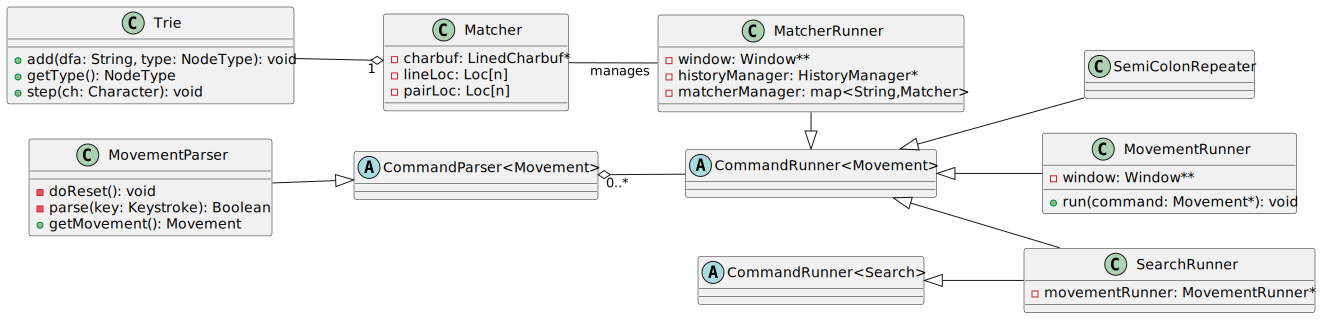
\includegraphics[width=\textwidth]{uml3}
\\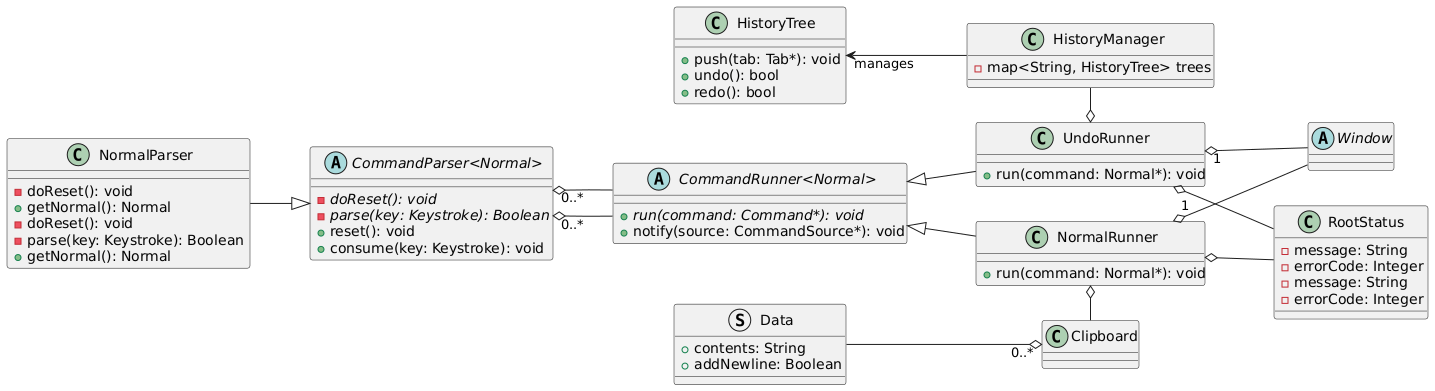
\includegraphics[width=\textwidth]{uml5}
\\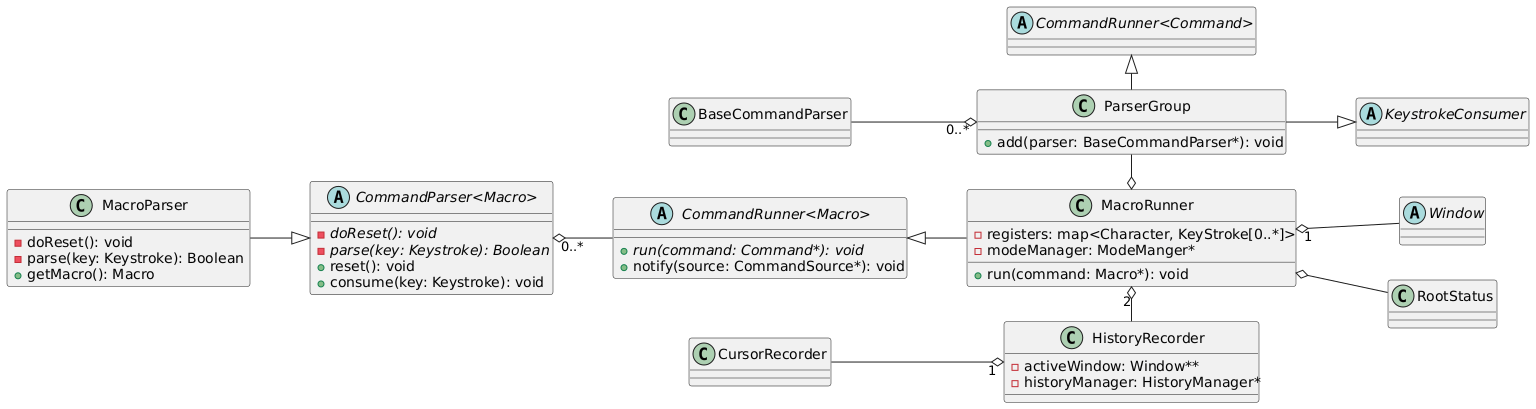
\includegraphics[width=\textwidth]{uml6}
Figure 3. Some selected parsers, runners, and model classes 
for implementing \texttt{ComboNM}, \texttt{Movement}, 
\texttt{Normal}, and \texttt{Macro} commands, in order from top to bottom. 
\\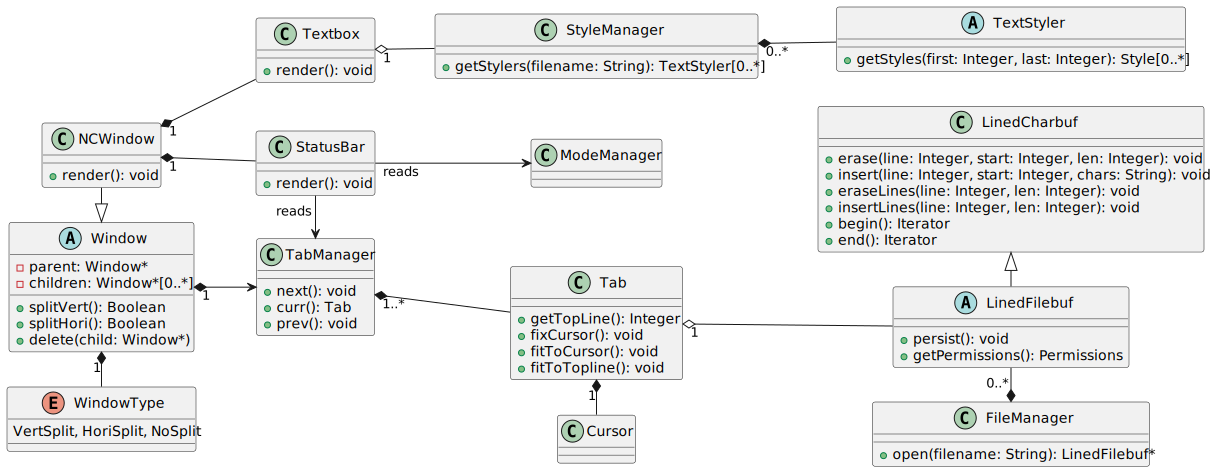
\includegraphics[width=\textwidth]{uml7}
Figure 4. Above: view classes \texttt{NCWindow}, \texttt{Textbox}, \texttt{StatusBar}, 
as well as model classes \texttt{Tab}, \texttt{LinedFilebuf}, 
their managers, and \texttt{Window}. 
Below: separated interfaces of above classes 
in order to adhere to interface segregation principle. 
\\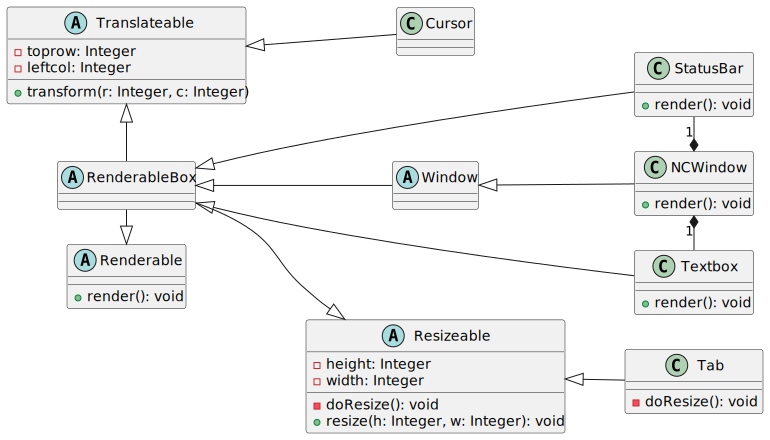
\includegraphics[width=250pt]{uml8}
\\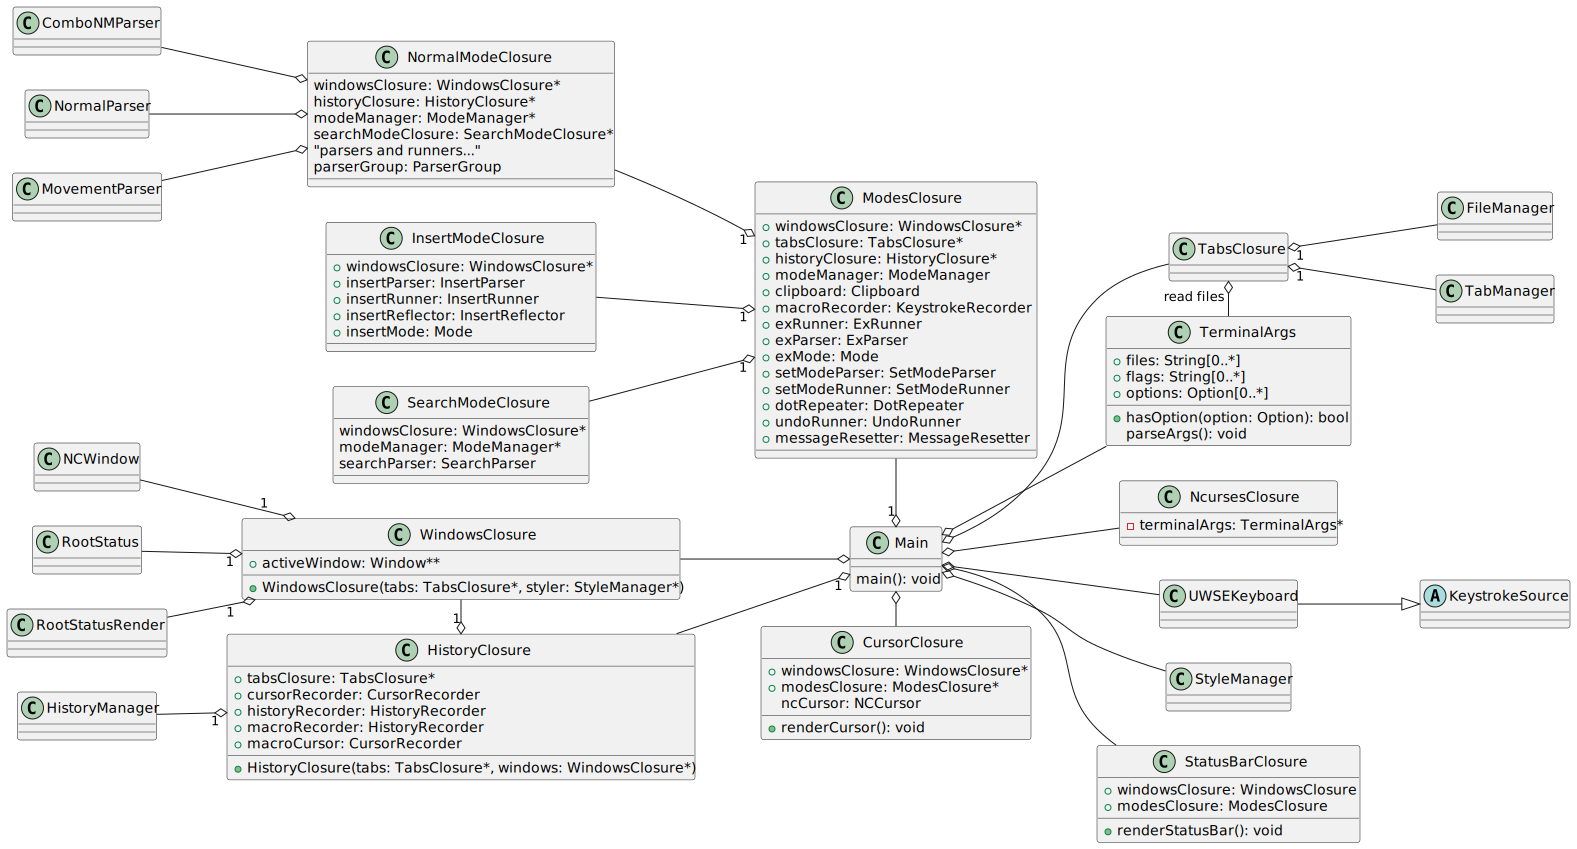
\includegraphics[width=\textwidth]{uml9}
Figure 5. Classes used in \texttt{Main} to RAII and initialize and attach 
all parsers and runners. 

\section{Design} 
\textbf{KeyStroke}: following MVC, I abstracted user input using  
the \texttt{KeyStroke} struct, along with enum \texttt{Key} to store its type. 
This increases Cohesion as all user-input related 
classes can be put in one module, and the rest of the model 
doesn't need to deal directly with user input. 
The slightly increased coupling from other classes needing to read from 
\texttt{KeyStroke} subjects is reduced by CRTP. 

\textbf{Command}: note that parsing and runnning commands should be separate. 
Hence, I added \texttt{Command} structs storing all info that could be parsed, 
and gave them parsers and runners. 
This increased cohesion by separating parsing from running, and commands from keystrokes. 
Note I decided on inheritance over variants, 
firstly because \texttt{Command}s differ a lot in size, so fixed-size variants 
are costly. More importantly, I can take advantage of covariant return types
so that in the parsers, \texttt{Command* getCommand()} can be overriden 
to return \texttt{Normal* getCommand()}. 
This becomes important in the \texttt{CommandRunner} section, 
and wouldn't be possible with variants. 

\textbf{Observer Pattern}: we skipped over Command pattern in lectures, 
so I improvised over observer pattern. I used this pattern twice: 
on \texttt{KeyStroke}s and on \texttt{Command}s. 
However, I differed from the textbook pattern in that 
I needed both to run without reading from its Subject: 
\texttt{ModeManager} should run \texttt{KeyStroke}s 
forwarded to it by \texttt{MacroRunner}, 
and all \texttt{CommandRunner}s need to run 
\texttt{Command}s forwarded by \texttt{DotRepeater} 
(the runner for normal-mode \texttt{.})
Furthermore, I noticed \texttt{notify()} methods 
mostly called \texttt{consume(subject.getKeystroke())} or \texttt{run(getCommand())}. 
\\Hence, I used CRTP on \texttt{Subject<State,S>} and 
with \texttt{Observer<S>}, where \texttt{S} is the subject 
(for examples, refer to \texttt{lib/keystroke/keystroke\_source.h}). 
Now, since \texttt{S} has a \texttt{getState()} method, 
we can specialize observers to call \texttt{getState()}
in its notify, instead of passing a reference to a concrete \texttt{Subject} 
in each conrete \texttt{Observer}. Overriding \texttt{notify} is still useful. 
For example, in \texttt{InsertRunner}, since the user already typed a copy of the insert, 
in \texttt{notify()} we repeat \texttt{count-1} inserts, 
while \texttt{DotRepeater()} calls it with \texttt{count} inserts. 
This design decreases coupling between consumers and runners, as they don't depend on 
the concrete subjects anymore. 

\textbf{CommandRunner}: I noticed most \texttt{CommandRunner}s 
were attached to one \texttt{Parser}, which only emits one type of \texttt{Command}, 
known at compile time. Hence, I templated runners and parser over 
the type of command they act on (e.g. \texttt{lib/command/runner/command\_runner.h}). 
This way, the \texttt{run()} method can take as argument a derived command type, 
and \texttt{notify()} takes a \texttt{CommandSource<Type>}, whose 
\texttt{getCommand()} returns the derived type so that \texttt{dynamic\_cast} is 
not required. Note that some runners (e.g. \texttt{JKRecorder}) 
should act on any type of command, 
hence I made \texttt{CommandSource<Command>}  a base class of all other 
\texttt{CommandSource}s. Covariant return types is necessary since 
we need to override getCommand in derived classes to return the derived type. 
This design 

\textbf{CommandParser}: To parse normal mode commands, 
I needed parsers to stop parsing if the keystroke is invalid, 
and be reset when one of the parseres succeededs, or they all fail. 
Hence, I created a \texttt{ParserBase} class inheriting \texttt{Resetable} 
and \texttt{KeystrokeConsumer}. 
This way, I can create a \texttt{ParserGroup} 
and preform homogenous actions over a collection of \texttt{ParserBase}s, 
e.g. checking if they are valid. 
Following interface templates, I made \texttt{consume()} \texttt{final} in the base 
and provided a private \texttt{parse()} method for subclasses to override. 
This way, parsers stop reading keystrokes when they fail. 

\textbf{Iterator Pattern}: I had \texttt{LinedFilebuf} extend from a \texttt{LinedCharbuf}, 
which implements a bidirectional iterator, and a reverse iterator. 
The \texttt{begin()} and \texttt{rbegin()} for these take a line and column 
marking the start point of the iterator. 
This is useful for searching movements such as 
\texttt{w,b,f,/,?,\%} and also helps with the \texttt{Textbox}, 
which uses the iterator to read and write chars. 
I decided to have iterators store line-col positions, which allows 
line-based arithmetic using pointers (useful for reading cursor position after searching).
To support constant time lookup, \texttt{LinedCharbuf} was represented as a \texttt{deque}
of \texttt{string}s, each terminated by a newline character. 
Hence, line-based operations like \texttt{dd} are constant time, 
and inserting within a line (i.e. insert mode) is linear in length of line 
(which is acceptable, as lines should be short). 
I noticed \texttt{line-col} pairs could be grouped into a \texttt{Loc} struct, 
and given an \texttt{operator<=>()} method to simplify comparisons 
(see \texttt{lib/matcher/matcher\_runner.h}). 

\textbf{Strategy Pattern}: to support search based movements, 
I wrote a \texttt{findNth} template over iterators (see \texttt{include/utility.h}) 
to return iterator to nth match within range of a \texttt{[beg,end)} pair of iterators, 
using a \texttt{Pred} (anything with \texttt{bool operator==(char)}) to find matches. 
I had the invariant that each character would be matched exactly once. 
Hence, implementing runners for search movements was: 
write a \texttt{Pred}, generate \texttt{[beg,end)} from the current cursor location, 
run \texttt{findNth}. Since iterators return their \texttt{Loc}s, 
it remains to set the \texttt{Cursor} location into the \texttt{Tab}. 
\\Some examples of \texttt{Preds} were \texttt{Chunk}s 
(\texttt{lib/command/runner/movement\_runner.h}), 
which I used to implement \texttt{w,b}. 
These store the previous character and uses it to check whether the current char
marks the end/start of a word. By the invariant of \texttt{findNth}, 
each \texttt{operator==} would update prev. 
Hence, I used mix-in inheritance to so that \texttt{Chunk} updates prev. 
Hence inheriting from it and overriding \texttt{doCheck} suffices. 
This allowed me to easily create \texttt{Chunk}s for \texttt{w,b,W,B}. 

\textbf{Word-Search}: Another \texttt{Pred} was for the \texttt{?,/} commands, 
for which I implemented a matcher using KMP string matching algorithm. 
I had the constructor generate a Longest-prefix suffix (LPS) array from the search string
that the user types into \texttt{Ex} mode, 
and move-assigned it to the matcher each time the user searches. 
Then, the \texttt{operator==} would match using the LPS. 
Reverse matching was implemented by constructing the LPS using the reversed string, 
and applying \texttt{findNth} using the reverse iterator 
obtained from \texttt{LinedCharbuf::rbegin()}. 

\textbf{Interface Segregation Principle}: 
note that many of the operations on \texttt{Tab}s, \texttt{Window}s, \texttt{Cursor}s
are similar. For instance, \texttt{resize}, \texttt{translate}, 
and \texttt{render}. Hence, I captured the first two into concrete classes 
\texttt{Resizeable}, \texttt{Translateable}, and \texttt{render} into 
the abstract \texttt{Renderable}. 
Note that some classes such as \texttt{Window}s need to recalculate 
their contents on \texttt{resize}. Hence, I used \textbf{NVI} on \texttt{Resizeable}, 
providing a private virtual \texttt{doResize()} for subclasses such as 
\texttt{Tab} and \texttt{Window}. 

\textbf{Open closed principle}: one specific instance I want to highlight 
which doesn't fit into existing patterns was the 
\texttt{Trie} class in \texttt{lib/matcher/matcher\_trie.h}. 
I implemented it so that any class could extend the DFA by 
\texttt{add()}ing branches as \texttt{string}s. 
Although the extension still requires modifying the \texttt{Node::Type} enum, 
the logic for stepping through the DFA is constant. 
Compared to the \texttt{CommandParser}s I wrote earlier on, 
this design is much more extensible. 
For example, to add support for matching \texttt{/*} and \texttt{*/}, 
I added two \texttt{add(...)} statements to the constructor, 
two cases to the enum, and two \texttt{case}s in the \texttt{Runner}'s switch statement. 
Note that the enum could be extracted into a hierarchy (similar to \texttt{Command}) 
or another module,
further increasing extensibility. 

\textbf{Prototype Pattern}: notice that a command like \texttt{c2w} 
is a \texttt{SetMode} command, since it activates insert after deteting 2 words. 
Hence, I decided to separate c + Movement commands into \texttt{CM}, 
which inherits from \texttt{SetMode}. 
However, for \texttt{DotRepeater} to play back an \texttt{Insert} command, 
it needs to also replay the logic from its preceeding \texttt{SetMode}. 
Hence, \texttt{DotRepeater} needs to copy construct \texttt{SetMode}s for future use 
(note that parsers are always reset after notifying, so cannot shallow copy its pointer). 
Hence, I gave \texttt{SetMode} a \texttt{clone} method, so that \texttt{CM} 
could be copied dynamically. 

\textbf{Justifications}: I justify implementing \texttt{Macro}s 
by recording and replaying keystrokes because that was easier than 
re-running a sequence of \texttt{Command}s 
(which would couple with all other runners). Instead, playing keystrokes into the 
the root \texttt{ModeManager} was simpler and more consistent. 
Furthermore, vim probably does this as well. Note that \texttt{:reg} 
shows recorded keystrokes (including \texttt{ctrl-G}), not commands. 
You can also change the keystroke recorded at a certain location. 
Hence vim macros are probably keystroke based. 
\\I justify managing history in a \texttt{tree} and storing snapshots 
of the entire file since I think vim also does the same 
(although they probably store file-deltas, rather than whole snapshots). 
Vim undo branches can be accessed via \texttt{:undolist} 
and allows you to go to any edit made during the editing session. 
I wanted to implement the same, although I ran out of time. 
However, my \texttt{HistoryTree} class does store undo branchs, 
as evidenced through GDB 
(set a breakpoint on line 40 of \texttt{lib/history/history\_tree.h}, 
watch \texttt{store}). 
\\Why is \texttt{LinedCharbuf} concrete? This violates dependency inversion principle. 
But in this case, 
I think of \texttt{LinedCharbuf} as an implementation of in-memory line-based operations, 
which won't change much in the specification if at all. 
\section{Extra-credit features}
\begin{myitemize}
  \item{Multifile - turn on(off) by ex command \texttt{:multifile on(off)}. 
    switch files with \texttt{:n}, \texttt{:N}. 
  This was difficult to design, since multiple files means 
  needing multiple cursors, window pane locations, etc. 
  I solved this using the concept of a \texttt{Tab}, 
and used \texttt{TabManager} to handle file switches. }
  \item{Help: type \texttt{./vm -h} for a help message. 
    I did this to show my extensions }
  \item{Colors: use \texttt{./vm --show-color --color-set standard } for colors. 
    I did this because it is pretty, and also error codes 
  (e.g. \texttt{:q} with unsaved changes) are highlighted}
  \item{Extended history: you can run \texttt{Ctrl+r} to redo commands. 
  I added this since I use it frequently, and is a simple first step towards undo-branches
   that I wanted to add (see \textbf{Justifications}). 
  I implemented this by storing undos into a "future stack", 
  and popping from the stack to redo. Pushing a new change clears the future. }
  \item{No explicit memory management: 
      I wanted this because it leads to cleaner, non-leaking code. 
    I achieved this using non-owning pointers, \texttt{unique\_ptr}s 
  and \texttt{std} library collections }
  \item{Extended movements: \texttt{W}, \texttt{B}. 
      These were extensions from \texttt{w,b}, 
      all of which I frequently use. 
    It also illustrates mix-in inheritance and strategy pattern well.
  See \textbf{Strategy Pattern}}
  \item{KMP pattern matching: allows for O(n+m) 
    plain-text searching. See \textbf{Word-Search}}
\end{myitemize}
3 additional features I'm not certain are enhancements but would like to highlight: 
1: Insert mode handles enter key (implemented because useful). 
2: Normal mode handles arrow key movements, and mouse scrolling. 
Supporing these is why I added the \texttt{Key} enum, which made it easy to extend. 
3: The \texttt{\%} matcher reproduces behaviour for \texttt{\#endif}, \texttt{\#if}, 
\texttt{\#elif}, \texttt{\#else}, \texttt{/*}, \texttt{*/}. 
This was difficult in that it required the \texttt{Trie} data structure
(see \textbf{Open closed principle}). 
\section{Final Question}
Based on the \texttt{Trie} class I wrote for \texttt{\%} runner, 
I would redesign the parsing of \texttt{Command}s 
so that each VM command's DFA path could be added via an \texttt{add} method, 
with exactly one \texttt{CommandRunner} corresponding to each \texttt{Command}. 
This would significantly decrease coupling, as each \texttt{Command} 
is isolated from others, and only commands such as \texttt{ComboNM} 
would rely on other Commands. 
This would make general runners such as \texttt{DotRepeater} 
extremely repetitive, although this can be addressed using the Command pattern. 
That is, we make \texttt{Command::run()} a pure virtual method, 
and initialize each \texttt{Command} with a \texttt{CommandRunner}. 
Since there's a bijection between Commands and Runners, 
concrete \texttt{Command}s can have a \texttt{static} member runner. 
Then, \texttt{concrete} \texttt{Command}s override \texttt{run} to 
pass themselves into the runner's run, along with data such as \texttt{count}, 
\texttt{register}, etc. 
This way, \texttt{DotRepeater} can just call \texttt{run()}, 
as can \texttt{ComboNM} runners. 
\\This was actually my original idea, however I could not figure out a reasonable 
way to represent a path, since one would need to parse \texttt{count}s, 
\texttt{register}s, and for \texttt{ComboNM}, multiple sub-DFA paths. 
Another disadvantage besides skill issue is that 
it would signficantly decrease cohesion,
since many VM commands are extremely similar. 
However, coupling is a far larger issue in this context. 
First, the side-effects from observer-pattern 
combined with parser-groups resetting themselves 
already make it very hard to reason about how commands run. 
Adding more commands would be nearly impossible, and having people collaborate 
would require a very long learning period. 
Furthermore, extending parser functionality currently requires modifying parser classes
(violating open-closed principle), whereas adding DFA paths leads to code that 
is cleaner, more efficient, and easier to reason about. 
Hence, I think the benefits outweight the duplicated code, 
and if the repetition is too bothersome, using mix-in inheritance can address the issue. 

\end{document}
